\section{Statistical Language Modeling}

\subsection{Problem overview}
%
%In general, language models aim at measuring the fluency of any text, showing how much it makes sense. Artificial systems that generate text, therefore, requires the aid of language models in order to produce textual outputs that are comprehensible. 

As we introduced before, the Statistical approach in Language Modeling aims at measuring the fluency of all possible word strings, which are considered as a stochastic process, with probabilities. The sequence length can be arbitrary, while the words are taken from a limited vocabulary. A trained language model should be able to show that the likelihood of "the end of our world" is much higher than "tea end of our word", because the latter string is much less likely to be found in available English text. Concretely, let us denote $W_1^L$ to be a word sequence with length $L$ which is composed by the constituent words $w_1,w_2,\dots,w_L$, then a statistical language model aims at predicting the probability distribution of all possible sequences $W_1^L$ in a particular language:

\begin{equation}
P(W_1^L) = P(w_1w_2\dots w_L)
\end{equation}

Since the direct estimation for that probability distribution is intractable, the probability of a sentence $P(w_1^L)$ is factorised using the chain rule:
\begin{equation}
\label{eq:lm1}
P(W_1^L) = P(w_1 | \text{\textless s\textgreater}) \prod_{i=2}^L P(w_i | \text{\textless s\textgreater} W_2^{L-1})\\
= \prod_{i=l}^L P(w_l | H_l)
\end{equation}
in which, \text{\textless s\textgreater} is used to denote beginning token of the sentence/string. The history $H_i$ represents the string before the current word $w_i$. Instead of directly modeling the original distribution, the target probability is factorised into constituent~\textit{conditional} probabilities, which are more practical to estimate. 
%
%The language modeling problem has experienced many approaches over the last two decades, most of which aiming at maximising the log-likelihood of the data (minimising the perplexity at the same time), while using some constraints and techniques to generalise to unseen data. The most widely used models rely on $n$-grams based on the Markov assumption that each word depends on $n-1$ previous words. 
%
%\begin{equation}
%\label{eq:markov}
%P(w_i|h_i) \approx P(w_i|w_{i-n+1}^{i-1})
%\end{equation}

\subsection{Evaluation Metrics}

The quality of statistical language models can be evaluated by the capability to predict a new corpus, which is defined by using~\textit{Perplexity}. Let us assume that we have a trained language model $M$ and a corpus $D$ containing $L$ words, which the language model has not observed during the training process. The quality of model $M$ is evaluated by using it to predict the distribution of the corpus $D$. The resulted perplexity~(PPL) is then obtained by estimating the probability of all words given their context in the corpus D, we use $P_M$ to denote the probability distribution produced by model $M$. An example of PPL computation is illustrated on Table~\ref{tab:examplePPL}.

\begin{equation}
\label{eq:ppl}
PPL(D) = \exp(\frac{\sum_{l=1}^L{-\ln P_M(w_i|H_i)}}{L}  )
\end{equation}


\begin{table*}
	\centering
	\begin{tabular}{|c|c|c|}
	\hline
	Word to be predict & Context & Probability (example) \\
	\hline
	The & \starts & 0.1 \\
	relationship & \starts The & 0.002 \\
	between & \starts The relationship & 0.05 \\
	Obama & \starts \dots relationship between & 0.00001 \\
	and & \starts \dots between Obama & 0.2 \\
	Netanyahu & \starts \dots Obama and & 0.00001 \\
	is & \starts \dots and Netanyahu & 0.05 \\
	not & \starts \dots Netanyahu is & 0.02 \\
	exactly & \starts \dots is not & 0.001 \\
	friendly & \starts \dots not exactly & 0.0007 \\ 
	. & \starts \dots exactly friendly & 0.2 \\
	\hline
	Perplexity & & 210\\ 
	\hline
	\end{tabular}
	\label{tab:examplePPL}
\caption{An example of perplexity computation for the sentence ``The relationship between Obama and Netanyahu is not exactly friendly''.}
\end{table*}

The idea of perplexity is that, minimising perplexity is corresponding to maximising the ability to predict every word in the data. A low perplexity value corresponds to the fact that the language model is able to fits better the data, since the distribution of the model is closer to the unknown distribution of the test data. One property of perplexity is that, it is correlated to the average number of guessing needed to predict all words in the data. Therefore, a random distribution or the ``worst'' model (usually the model with parameters initialised) often gives the perplexity very close to the vocabulary size $V$. This property is often used to check the implementation of the model and perplexity. 

In practice, the quality of language models can also be evaluated through their impacts on other applications such as Automatic Speech Recognition (ASR) or Statistical Machine Translation (SMT), by reducing the errors in the output of such systems. For example, two strings ``Tea end of our word'' and ``The end of our world'' may have similar speech signals and the recognizer has to rely on a good language model to distinguish them. 

The main advantage of perplexity is that it is fast to perform and independent to other complex systems. Therefore, in this thesis, PPL would be the only measurement used in the experiments. However, it is important to note that an improvement in terms of perplexity does not always result in the application improvement. For example, the improvement is required to be at least $10\%$ to be noteworthy for an ASR system~\cite{Rosenfeld:2000}. Also, there are some language models that aim at ranking the words in the vocabulary by using unnormalised distributions (the sum of the probabilities does not equal to $1$). In that case, PPL is also unusable. 


\subsection{$N$-gram models}

Going back to equation~\ref{eq:lm1}, the target of statistical language models is to estimate the conditional probabilities $P(w_i|H_i)$ with $H_i$ being the history context of $w_i$ ($i$ is an arbitrary index in the corpus). A common approach is to limit the length of the history $H_i$ by the Markov assumption: the meaning of the word $w_i$ only depends on $n-1$ words before, thus limiting the history for all words in the data into $n$-grams:

\begin{equation}
P(w_i|H_i) \approx P(w_i | W_{i-n+1}^{i-1}) 
\label{eq:ngram}
\end{equation}

With $W_j^k$ denotes the word sequence from index $j$ to index $k$. It is natural to use $n-1$ to denote the order of language models because it is the order of the Markov model reflected in Equation~\ref{eq:ngram}, however in the literature, authors always use $n$ to denote the order of $n$-grams. Therefore, in order to be clear, an $n$-gram contains one word to be predicted, and $n-1$ words in the context. 

Count-based models estimate the probability of each $n$-gram based on simple counting with maximum likelihood estimation. Let $c(W_j^i)$ denote the number of times that this word sequence occurs, the estimated distribution can be derived as follows:

\begin{equation}
P(w_i | W_{i-n+1}^{i-1}) = \frac{c(W_{i-n+1}^{i})}{c(W_{i-n+1}^{i-1})}
\label{eq:ngram2}
\end{equation}

The method is unreliable since it struggles at estimating the distribution for rare and unseen $n$-grams (the nominator is 0), many of which actually make sense in natural language. Many techniques have been proposed to overcome this weakness, from re-distributing the probabilities of the frequent $n$-grams to the less frequent ones (smoothing techniques) or deriving the distributions of the rare $n$-grams from the lower order $n$-grams (interpolation and back-off techniques)~\cite{kneser1995improved,chen1999empirical,heafield2011kenlm,federico2008irstlm,ney1994structuring,witten1991zero}. However, even with complicated smoothing techniques, the main weaknesses of $n$-gram language models are still exposed as follows:

% 2. Weakness 
First, each word in the vocabulary is treated as a totally discrete random variable without any linguistic feature associated. The model relies on statistical occurrences and ignores morphological, syntactic and semantic relationship, by which the lexicon is formulated. There are several attempts to incorporate the word similarity in $n$-gram based language models. Notably, the class-based language models~\cite{brown1992class,niesler1996variable} introduced word clustering and assumed that the distribution of unseen or rate words can be achieved by using the richer statistics from the corresponding class, which is less sparse than the word itself. Also, the structured language models~\cite{chelba2000structured,filimonov2009joint} tries to filter out irrelevant context words and focuses on important counterparts by using parse trees, which compensates the lack of syntactic information in $n$-gram models. Despite such efforts, the language modeling results were still unreliable compared to the Knesey-Ney smoothing technique. However, those works in the literature also suggests that the syntactic and semantic properties of words need to be automatically learned from the data. 
%
Second, $n$-gram language models struggle to model a long range dependency between the predicted word and the context. Due to the fact that each word in the vocabulary is a separated random variable, the number of parameters to be estimated (statistics of $n$-grams) grow exponentially with the size of context. The~\textit{the curse of dimensionality} refers to the fact that one needs more amount of training data in order to reliably estimate the model when the number of learned parameters increases. For example, if the vocabulary size is $10000$, the total number of $n$-grams for $n=6$ is $10^16$ theoretically, which is also the number of parameters to be estimated accordingly. Also, the Zipf's law~\cite{kingsley1932selective} indicates that only a small subset of the vocabulary accounts for most occurrences in the training data, thus it is almost impossible to have a training data that covers all possible $n$-grams. 

The neural network language model, as a consequence, is investigated in order to tackle both problems that traditional count-based models cannot solve. 


\section{Neural Network Language Models}

In this section, we describe the neural language models (also known as continuous space language models), which are designed to fight the curse of dimensionality in the conventional approaches, by utilising two properties as follows
%In order to fight the curse of dimensionality described above, neural language models are designed to utilise two properties as follow:

\begin{itemize}
	\item Words are no longer discrete variables without any relationship to each other. Alternatively, they are represented as real-valued vectors in a continuous space, where similar words are neighbors in the space, such approach is referred as~\textit{Distributed word representation} or~\textit{Word embedding}~\cite{bengio2003neural,mikolov2010recurrent}. With such representation, each $n$-gram is a combination of the word vectors and $n$-grams with similar words share the same word vectors.  In contrary to the count-based approach, if we increase the $n$-gram order then thanks to the sharing property, we just need to adjust the size of the context vector, which can grow linearly with the $n$-gram order (in the case of feed-forward neural networks) or remains the same (in the case of recurrent neural networks).
	
	\item When the $n$-gram context $H_i$ is the combination of the word vectors, the conditional probability distribution $P(w_i|H_i)$ of each $n$-gram is then expressed as a parameterised smooth function of the context vector. In machine learning, neural networks are a class of models that can be used to approximate functions. As a result,~\newcite{bengio2003neural} proposed to incorporate the continuous word space with a neural network architecture in order to learn the smooth function. The training methods of neural network allow us to~\textbf{jointly learn} the word space and the parameters of that probability function. 
\end{itemize}

In the following, we provide the detailed description of two most successful architectures used for neural language models: the feed-forward models and the recurrent models.



\subsection{Feed-forward neural language models}



The standard architecture of a neural language model~\cite{bengio2003neural} is illustrated in Figure~\ref{fig:neuralBengio}. The model takes the context words $H_i$ as inputs and outputs the conditional probability distribution over~\textit{all} words in the vocabulary which expresses $P(w_i|H_i)$. It consists of three basic components: the input layer, the hidden layer and the output layer. The notations are covered in Table~\ref{tab:notationFFNN}. In a standard feed-forward neural network, each layer is a real-valued ~\textbf{vector}, while the (learnable) weights (or parameters) are real-valued~\textbf{matrices} connecting the layers together. Also, in the standard architecture we also consider networks with only one hidden layer for ease of understanding. In practice, it is possible (and beneficial) to extend the network with multiple hidden layers.


\paragraph{Input layer}
The input layer constructs the embeddings of the words in the context, by using a shared word space and mapping each word in the context to a real-valued vector. Concretely, each word $w_i$ is represented as an 1-of-V coding, which is a long vector with the size of vocabulary V with all zeros except for the element corresponding to the word's index in the dictionary. Using this form of sparse coding, the word space (also called projection matrix $R$) is a matrix that contains V rows and each word embedding $v_i$ corresponds to one row of the matrix. The number of columns of the matrix is the size of the embedding, which is a tunable hyper-parameter. Notably, the values of the word vectors do not depend on the position of the word in the context. The context vector $i$ is the concatenation of the word vectors.

~ \begin{figure}[!t]
	~ \centering
	~ 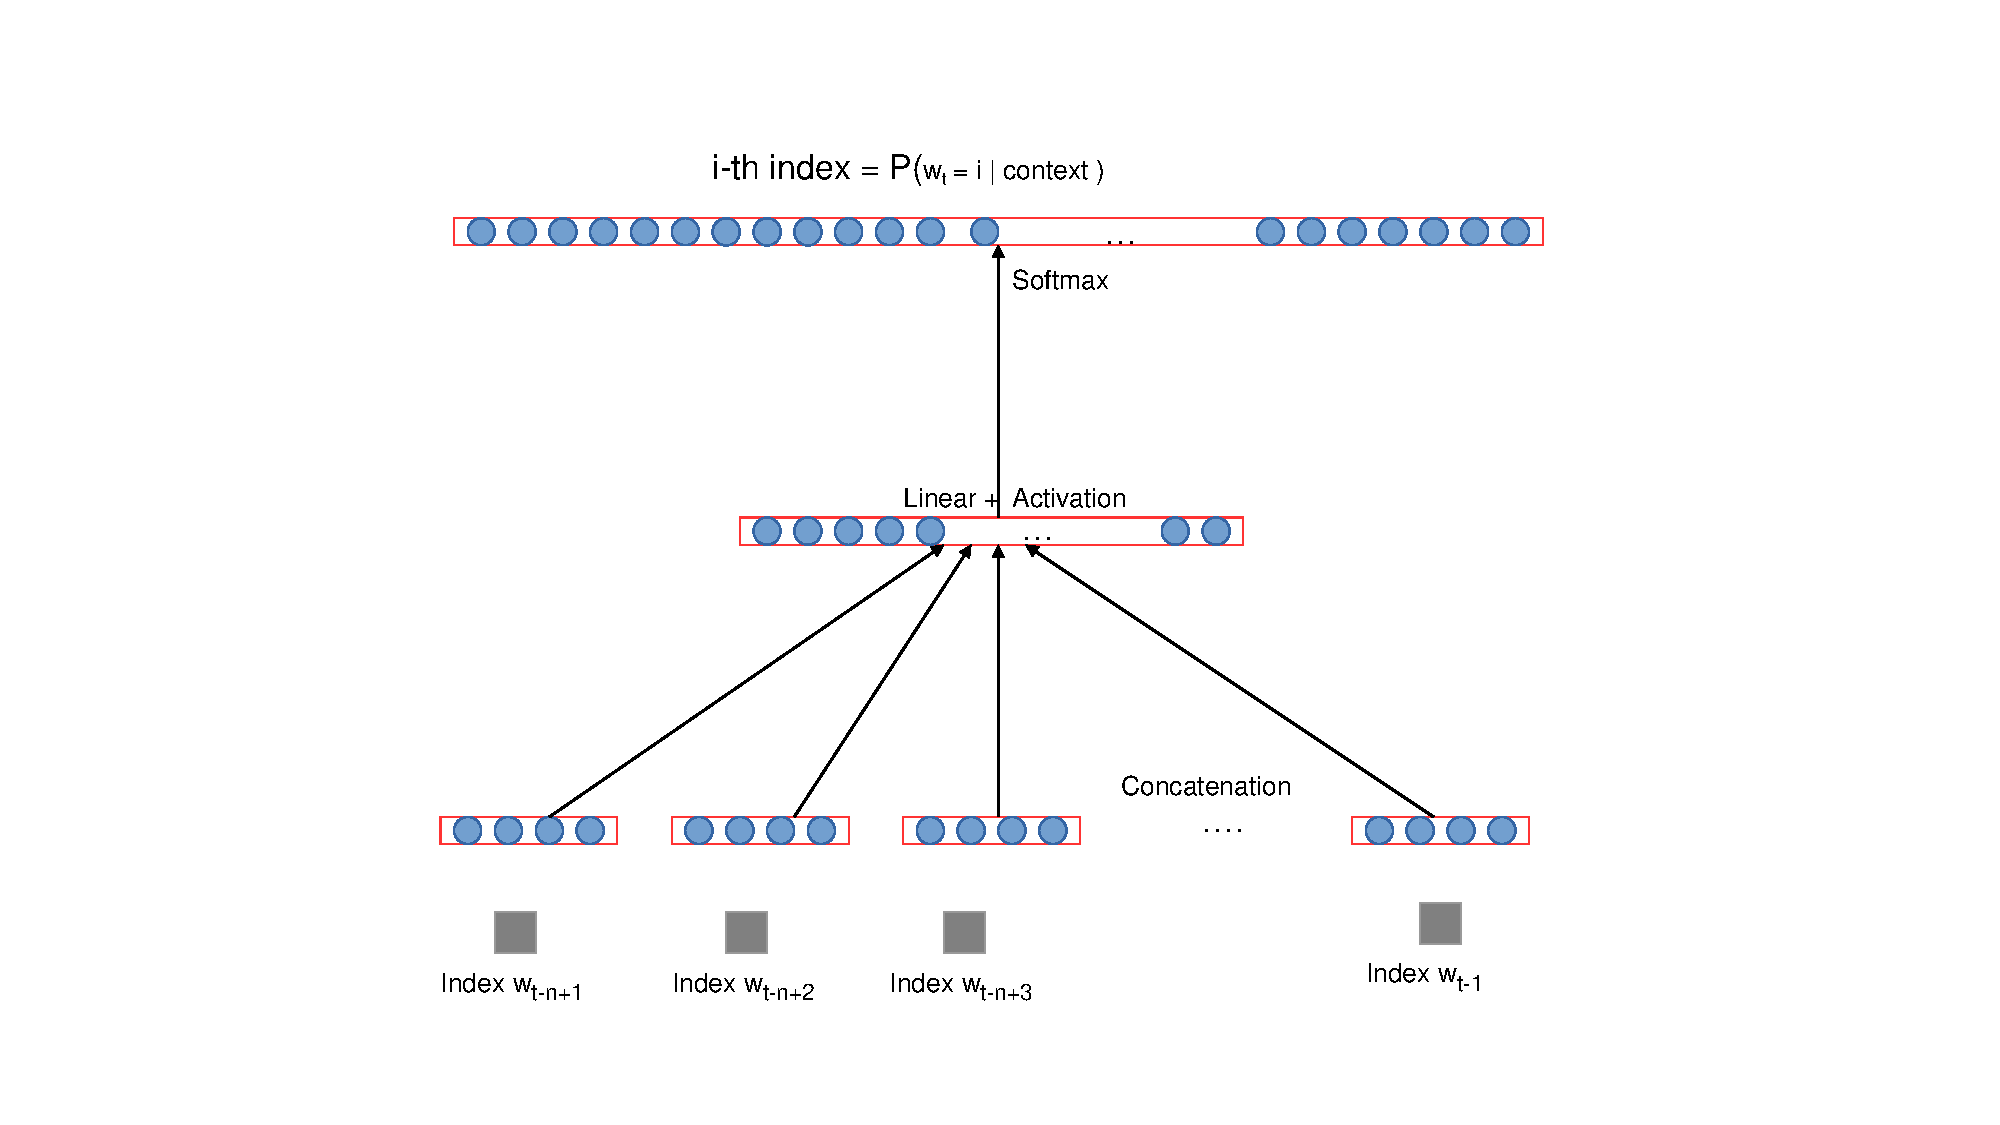
\includegraphics[width=\columnwidth]{figures/neuralLM.pdf}
	~ \caption{Neural Language Model by Bengio et al~\cite{bengio2003neural}.}  
	~ \label{fig:neuralBengio}
	~ \end{figure}

\begin{table*}
	\centering
	\begin{tabular}{|c|p{10cm}|}
		\hline
		notation & meaning \\
		\hline
		$V$ & Vocabulary size \\
		$m$ & word vector dimension \\
		$n$ & order of language model \\
		$w$ & a word; its index in the vocabulary \\
		$v_w$ & one-hot vector for word $w$. A vector with size $V$ with all null except the $w^{th}$ index (=1) \\
		\hline
		$i \in \mathbb{R}^{(n-1)M}$ & input vector of the network. \\
		$o$ & output layer of the network which expresses the \newline unnormalised probability distribution \\
		$h$ & hidden layer of the network \\
		$p$ & the output vector of the network which is normalised for the \newline conditional probability distribution \\
		$i_j$ & the $j^{th}$-index of vector $i$, which is also used for $o, h \text{ or } p$ \\
		\hline
		$f$ & nonlinear function \\
		$H$ & hidden layer size \\
		$W^h \in \mathbb{R}^{H \times (n-1)M}$ & the weight matrix connecting \newline the input layer with the hidden layer \\
		$b^h \in \mathbb{R}^H$ & the bias vector for the hidden layer \\
		\hline 
		$W^o \in \mathbb{R}^{H \times V}$ & the weight matrix connecting \newline the hidden layer with the output layer \\
		$b^o \in \mathbb{R}^V$ & the bias vector for the output layer \\
		\hline
		$\mathcal{L}$ & The objective (loss) function for learning the network \\
		$dX$ & The Jacobian matrix - the matrix of all of the first order partial derivatives of the loss function with respect to the vector/matrix $X$. \\
		\hline
	\end{tabular}
	\label{tab:notationFFNN}
	\caption{Notations for neural network layers.}
\end{table*}

\begin{equation}
\begin{aligned}
i = \{R^T v_1; R^T v_2; .... ; R^T v_{n-1} \}
\end{aligned}  
\end{equation}


\paragraph{Hidden layer}
In the hidden layer, the input (context vector) is transformed nonlinearly, where each layer activation values are defined by

\begin{equation}
\begin{aligned}
h = f(W^h i + b^h) \\
\label{eq:hidden1}
\end{aligned}  
\end{equation}

In equation~\ref{eq:hidden1}, the hidden layer $h$ has the corresponding weights $W^h$ and $b^h$. The input of the hidden layer is the context vector produced from the input (projection) layer. The size of the hidden layers are tunable hyper parameters. $f$ denotes a nonlinear activation function. Popular choices for the activation function are Tangent Hyperbolic, Sigmoid or ReLU, expressed in equation~\ref{eq:activation}. 


\begin{equation}
\begin{aligned}
f(x) = 
\begin{cases}
\frac{\exp (x) - \exp (-x)}{\exp (x) + \exp (-x)}    \text{    if } f = \text{Tanh} \\
\frac{1}{1 + \exp(-x)}                \text{     if } f = \text{Sigmoid} \\
\max(0, x) \text{     if } f = \text{ReLU} \\
\end{cases}
\label{eq:activation}
\end{aligned}
\end{equation}

\paragraph{Output layer}
The final layer of the network produces the probability distribution for all words in the vocabulary, thus having totally V nodes. Each neuron in the layer is associated to the probability of one word, as shown in Figure~\ref{fig:neuralBengio}. First, a linear transformation is used to obtain the unnormalised distribution:

\begin{equation}
\begin{aligned}
o = W^o h + b^o
\label{eq:linearoutput}
\end{aligned}  
\end{equation}

Notably, the values of $o$ is unnormalised because each element in o is associate to the score of each output word given the context vector. $W^o$ and $b^o$ are the corresponding weights and biases of the layer. Importantly, $W^o$ has the same form as the projection matrix at the input layer, since it also learns embedding for each word in the output vocabulary. Subsequently, the true probability distribution is estimated thanks to the~\textit{softmax} function:

\begin{equation}
p(w_i | h) = \frac{\exp(o_i)}{\sum_j \exp(o_j)}
\label{eq:softmax}
\end{equation}

In equation~\ref{eq:softmax}, the probability of each word $w_i$ given the encoded context $h$ is estimated by normalizing all values in $o$. Overall, the main tunable hyper-parameters of the network are the order of $n$-grams (the number of words in the context, which can range from 6 to 15), the sizes of hidden layers, and the word embedding size. The set of free parameters~$\Theta$ that are iteratively updated by learning from the data includes the projection matrix $R$, the weight matrices $W^h$ at the hidden layers, $W^o$ at the output layer and the biases $b^h$, $b^o$. 


\subsection{Training method}
From the machine learning perspective, the neural network language model has transformed the statistcal language modeling problem from a generative learning process to a discriminative classification problem. The free parameters of the network are trained by minimising the objective function, which is the log-likelihood~$\mathcal{L}$ of the  parameters~$\Theta$ given the training samples. The parameters are updated after each iteration based on some optimization techniques, among which Stochastic Gradient Descent (SGD) is most commonly used in neural language models~\cite{zaremba2014recurrent,le2011structured,mikolov2010recurrent}. SGD and other variants such as Adadelta~\cite{zeiler2012adadelta} or RMSProp~\cite{tieleman2012lecture} require the computation of the first order derivatives of the loss function with respected to the parameters, which can be performed efficiently with the back-propagation algorithm~\cite{le1990handwritten}.

\subsection{Optimisation Process}
In this section, we describe the back-propagation flow in the standard feed forward neural language model - the core of the optimisation process. Back-propagation~\cite{rumelhart1985learning} involves using a dynamic programming strategy to compute the derivatives of the loss function with respect to the parameters layer by layer, based on the chain rules. In the standard network, the error derivatives are back-propagated from the output layer to the input (projection) layer.

\paragraph{Objective Function}


The smoothing function that we approximate with the neural network has parameters that can be iteratively tuned in order to~\textbf{maximise the log-likelihood of the training data}~\cite{bengio2003neural}. The objective function is therefore chosen as the Negative Log-Likelihood function, since SGD requires the training objective to be minimised. Assuming we have N samples in the training data, each of which is an $n$-gram, we can compute the loss function over the training data as follows:

\begin{equation}
\mathcal{L} = - 	\sum_{i}^N \log P( w_i | w_{i-n+1}^{i-1} ) \\
\label{eq:objective}
\end{equation}

The loss function is also in line with the Perplexity in Equation~\ref{eq:ppl}. For ease of understanding, we denote the derivative of the loss function~$\mathcal{L}$ at~\textit{each} sample or mini-batch of samples with respect to a variable $x \in \Theta$ by $dx$.  

For each sample $w_i$ and its context $H_i$, we have:

\begin{equation}
\begin{aligned}
- \log P(w_i |  w_{i-n+1}^{i-1})  = - \log P(w_i | H_i) \\
= - log (\frac{\exp (o_w)}{\sum_i exp(o_i)}) \\
=  log(\sum_i \exp(o_i)) - o_w
\label{eq:objective2}
\end{aligned}
\end{equation}

Subsequently, we compute the error derivatives $dx$ given the parameters in each layer using back-propagation:

\paragraph{Output layer}

The derivatives at the output layer:

\begin{equation}
do_i = 
\begin{cases}
1 - p_i \text{ if } i == w \\
-p_i \text{     otherwise}
\end{cases}
\end{equation}

Notably, $o_i$ denotes the $i^{th}$ element of the vector $o$, which is the unnormalised conditional distribution of the vocabulary given the encoded context $h$. 

\paragraph{Hidden layers}
As a result, we can compute the derivatives with respect to the parameters and the previous hidden layer $h$, based on the original inference from Equation~\ref{eq:linearoutput}. 

\begin{equation}
\begin{aligned}
dW^o = doh^T \\
db^o = do \\ 
dh = {W^o}^Tdo \\
\end{aligned}
\end{equation}

%
%For the inner hidden layers, the  derivatives for the linear components are computed similarly, by replacing $do$ with $dh$ (the output of the previous hidden layer is the input of the next hidden layer). However, we have to take into account the non-linear activation functions, which are shown in the inference equation for the previous hidden layers:
%
%\begin{equation}
%h_{next} = f(W^h h_{prev} + b^h)
%\end{equation}
%
%With $W^h$ and $b^h$ are the corresponding weights connecting $h$ to $o$. The derivatives are computed as follows:

%\begin{equation}
%\begin{aligned}
%d[W^h h_{prev} + b^h] = f'(h_{next}) dh_{next} \\
%db^h = d[W^h h_{prev} + b^h] \\
%dW^h = d[W^h h_{prev} + b^h]h_{prev}^T \\
%dh_{prev} = {W^h}^T d[W^h h_{prev} + b^h]
%\label{eq:dhidden}
%\end{aligned} 
%\end{equation}

%The derivative for $f$, $f'$:



\paragraph{Input Layer}

The inference equation for the hidden layer from the input layer:

\begin{equation}
\begin{aligned}
h = f(W^h i + b^h) \\
\label{eq:hidden1}
\end{aligned}  
\end{equation}

which implies that:

\begin{equation}
\begin{aligned}
d[W^h i + b^h] = f'(h) * dh \\
db^h = d[W^h i + b^h] \\
dW^h = d[W^h i + b^h]i^T \\
di = {W^h}^T d[W^h i + b^h]
\label{eq:dhidden}
\end{aligned} 
\end{equation}
%
%The derivative function of the input layer is identical to Equation~\ref{eq:dhidden} and Equation~\ref{eq:dactivation}, considering that the input layer is the layer before the first hidden layer. 

In order to have the derivatives for the activation function $f$, we have:

\begin{equation}
\begin{aligned}
f'(x) = 
\begin{cases}
1 - \text{Tanh}(x)^2   \text{    if } f = \text{Tanh} \\
\text{Sigmoid}(x) - \text{Sigmoid}(x)^2                \text{     if } f = \text{Sigmoid} \\
1 \text{ when } x > 0 \text{ and 0 otherwise}  \text{     if } f = \text{ReLU} \\
\end{cases}
\label{eq:dactivation}
\end{aligned}
\end{equation}

\paragraph{Parameter Update}

After obtaining the derivatives of the loss function with respect to all parameters in the network, we can update the parameters following to Stochastic Gradient Descent. The method is based on the phenomenon that the gradient of a function always points towards the direction of maximal increase at any point. The update rule is as follows with the learning rate parameter $\alpha > 0$ and an arbitrary parameter $x$:

\begin{equation}
x = x - \alpha dx
\label{eq:sgd}
\end{equation}

The learning rate is also considered as a function of the number of samples trained in the data. From experiments, the learning rate is updated after the model observes a number of training examples with two typical ways. The first way is to exponentially decrease the learning rate after some training samples with a~\textit{learning rate decay}, normally an epoch (training all samples in the training data). The second way is to reduce the learning rate based on a validation data. After each epoch, if the perplexity on the validation data is decreased, the learning rate is kept the same, otherwise it is multiplied by the learning rate decay.

\paragraph{Methods to prevent overfitting} Overfitting is a phenomenon that the model has poor predictive performance, even if the model is well trained on the training data. The possibility of overfitting exists because the criterion used for training the model is different than the criterion used to measure the efficacy of the model. It is very likely that the training data yields a different distribution than the test data, therefore fitting the model on the training data does not guarantee a good prediction performance. 

For neural network language models, the main methods used to prevent this phenomenon to happen is to apply~\textbf{regularisation methods} and~\textbf{early-stopping} strategy. 

\begin{itemize}
	\item Regularisation: The most efficient method is to apply~\textbf{Dropout technique}, which refers to dropping out units (in most case, hidden units) in neural networks~\cite{hinton2012dropout,srivastava2014dropout}. Concretely, we temporarily set the unit values to $0$ based on a random distribution (Bernoulli distribution, for example) during the training phase. In the testing phase, the unit is always present. Dropout is usually applied in the hidden layers of feed-forward neural networks. The choice of which unit to drop in the layer is random which is normally associated with a fixed probability $p$ independent for each unit. Depending on the network size and the amount of training data, the value of $p$ is chosen empirically.
	
	\item Early-stopping: In order to prevent overfitting, we use a validation set during training. The validation data is a separate set with the size similar to the test data. After each epoch (normally a whole scan over the training data), we measure the perplexity of the model on the validation data. If the perplexity does not decrease, the learning rate is reduced in the next epoch. The training process is halted when the learning rate reaches a threshold.
\end{itemize}
 
\subsection{Recurrent neural language models}

Compared to the statistical $n$-gram models, the feed-forward neural language models had created a considerable leap in representation by combining distributed representation of words with a robust classifier to generalise from observed sequences. As can be seen from various works~\cite{schwenk2007continuous,le2011structured}, the feed-forward language model significantly outperformed the traditional count-based models. However, the feed-forward models require a fixed input size, thus still rely on the Markov Assumption which limits the context to a particular number of words, even when the context size can be large. In order to model long sentences, or even paragraphs with long-term dependencies, it is beneficial to investigate in models that can be flexible in terms of input size. For example, if the distance between the open bracket and the closed counterpart is further than the $n$-gram input size, the feed forward model may forget to close the brackets after seeing the initial one. Ideally, as the learning process of human is associated with a memory that keeps the current information (such as topics), similar structure should be simulated and integrated in the network.

\paragraph{Recurrent Neural Networks} RNN~\cite{elman1990finding} are a class of neural networks that can efficiently model sequences by using a dynamic memory structure. While the feed-forward network can only receive one input and compute the corresponding output without any relation with other inputs, the recurrent counterpart takes the input as a~\textit{series of time step}  $x_1, x_2, \dots, x_n$ and processes them one by one, taking into account the information stored in the previous steps. Concretely, for each input $x_i$, the network updates the hidden memory $h^i$ based on the previous one $h^{i-1}$. 

%The ''Vanilla`` model~\cite{elman1990finding} uses a simple combination of the input and the previous memory:

\begin{equation}
h^i = \mathcal{F}(x_i, h^{i-1})
\end{equation}

We will cover some popular RNN variations in the upcoming sections. In general, the strong point of these models lie in the ability to dynamically model sequences with arbitrary length, which the feed-forward neural networks cannot achieve. The advantage comes with the cost that the recurrent models are generally hard to train, due to the properties of back-propagation. A change in an arbitrary position of the sequence can lead to a change in the objective function, therefore training methods for RNNs typically have to trace back the previous time steps. In other words, the RNNs are equivalent to feed-forward neural networks with many hidden layers that share parameters across each other. Importantly, the model capacity of RNNs do not depend on the length of the sequences, but in the recurrence mechanism - the way the hidden layers are updated. 

\paragraph{Recurrent Language Models} Language Modeling can be viewed as a sequence modeling problem, in which each time step corresponds to one word. We reuse the notations from Table~\ref{tab:notationFFNN} with another notation for recurrent layers added by Table~\ref{tab:notationRec}

\begin{table*}
	\centering
	\begin{tabular}{|c|p{10cm}|}
		\hline
		notation & meaning \\
		\hline
		$V$ & Vocabulary size \\
		$M$ & word vector dimension \\
		$n$ & order of language model \\
		$w$ & a word; its index in the vocabulary \\
		$H$ & hidden layer size \\
		$v_w$ & one-hot vector for word $w$. A vector with size $V$ with all null except the $w^{th}$ index (=1) \\
		$X^T$ & the matrix / vector X transposed \\
		$X * Y$ & The element-wise matrix multiplication between matrices $X$ and $Y$\\
		\hline
		$i^t \in \mathbb{R}^{M}$ & input vector of the network at time $t$. \\
		$h^t \in \mathbb{R}^{V}$ & hidden layer of the network at time $t$ \\
		$o^t \in \mathbb{R}^{V}$ & output layer of the network which expresses the \newline unnormalised probability distribution at time $t$\\
		$p^t \in \mathbb{R}^{V}$ & the output vector of the network which is normalised for the \newline conditional probability distribution \\
		$f$ & nonlinear function \\
		$W^i \in \mathbb{R}^{H \times M}$ & the weight matrix connecting \newline the input layer with the hidden layer \\
		$W^h \in \mathbb{R}^{H \times H}$ & the weight matrix connecting the hidden layer of the previous step \newline  with the current hidden layer \\
		$b^h \in \mathbb{R}^H$ & the bias vector for the hidden layer \\
		\hline 
		$W^o \in \mathbb{R}^{H \times V}$ & the weight matrix connecting \newline the hidden layer with the output layer \\
		$b^o \in \mathbb{R}^V$ & the bias vector for the output layer \\
		\hline
		\hline
		$\mathcal{L}$ & The objective (loss) function for learning the network \\
		$dX$ / $dx$ & The Jacobian matrix - the matrix/vector of all of the first order partial derivatives of the loss function $\mathcal{L}$ with respect to the matrix $X$ or vector $x$. \\
		\hline
	\end{tabular}
	\label{tab:notationRec}
	\caption{Notations for recurrent neural network layers.}
\end{table*}


The first recurrent language model (RNNLM)~\cite{mikolov2010recurrent} employed the ``Vanilla'' model of Elman et al~\cite{elman1990finding} as can be seen in Figure~\ref{fig:SimpleRNN}, in which the hidden steps are updated as follows:

~ \begin{figure}[!t]
	~ \centering
	~ 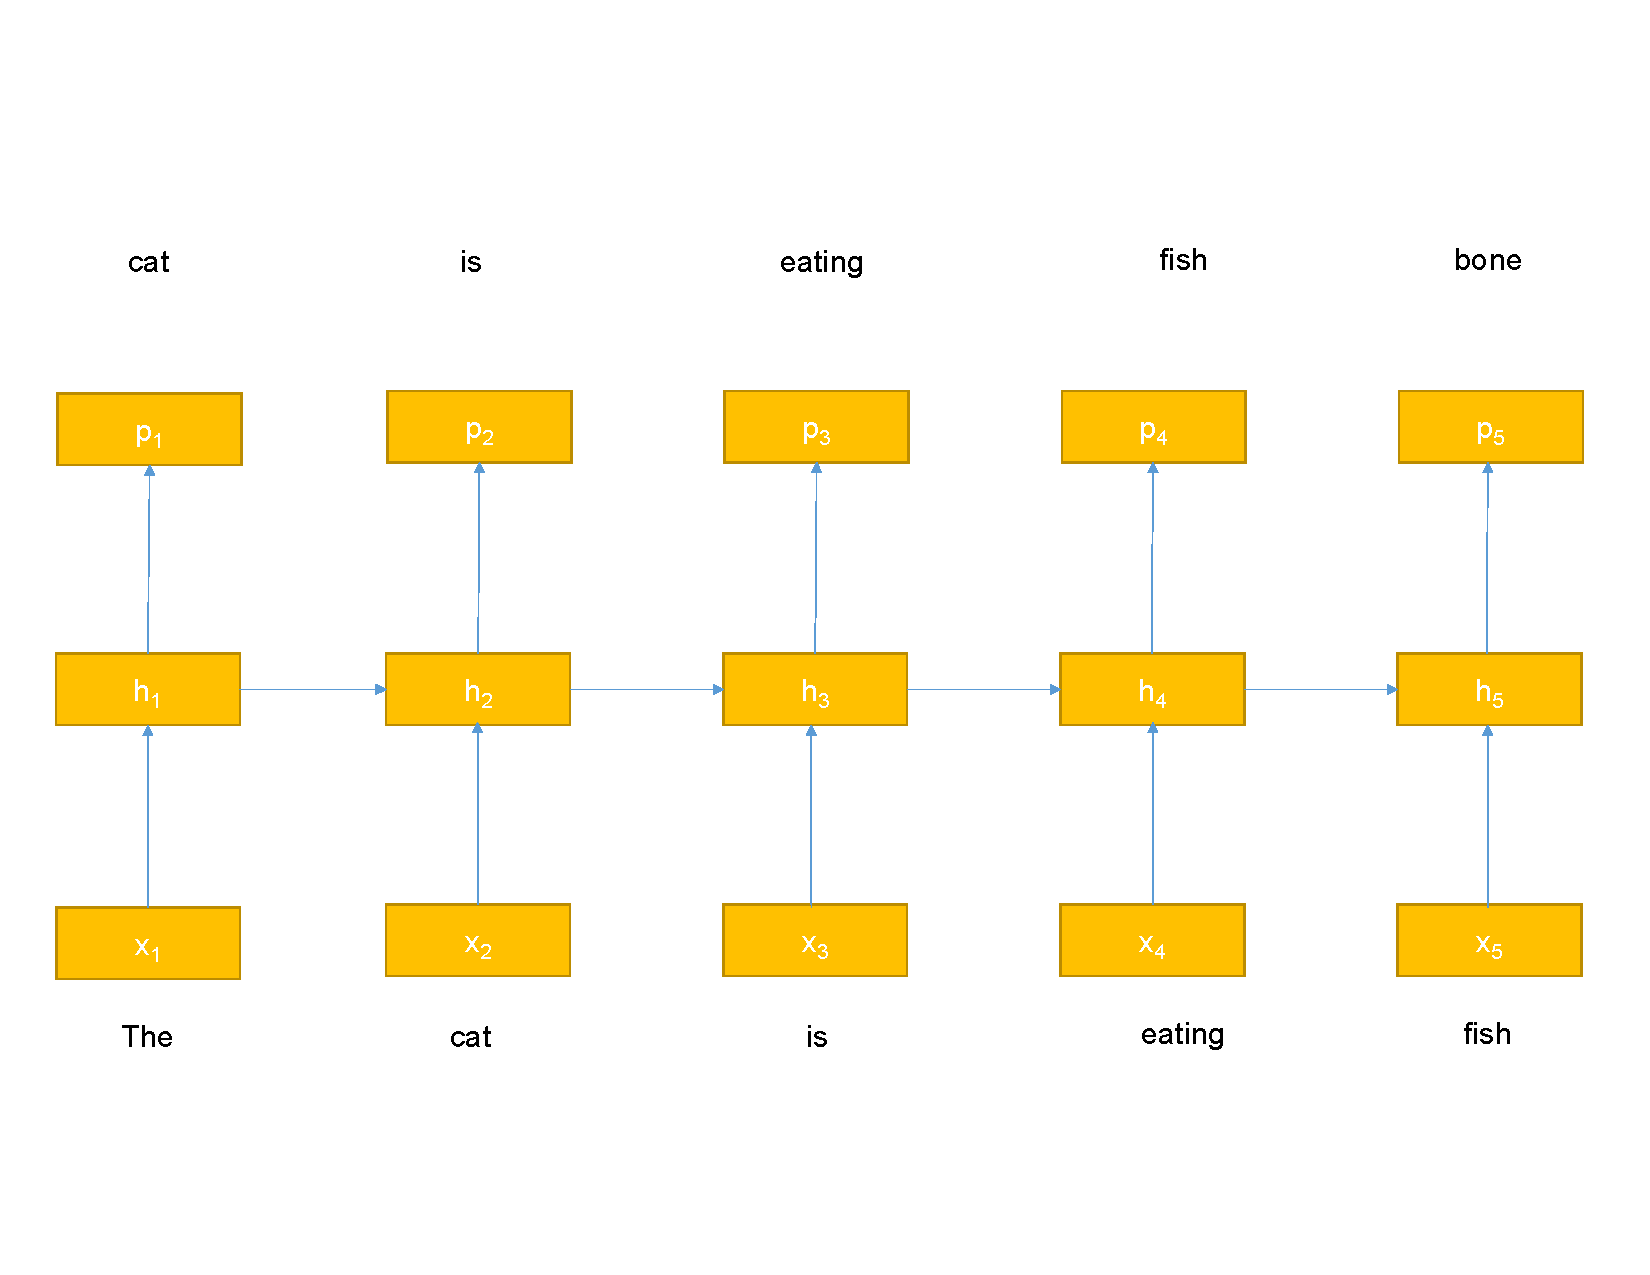
\includegraphics[width=\columnwidth]{figures/rnn.pdf}
	~ \caption{A simple RNNLM~\cite{mikolov2010recurrent} predicting the sequence ``The cat is eating fish bone''.}  
	~ \label{fig:SimpleRNN}
	~ \end{figure}


\begin{equation}
h^t = f(W^i i^t +  W^h h^{t-1} + b^h)
\label{eq:rnnhidden}
\end{equation}

The activation function $f$ can be either Tangent Hyperbolic, Sigmoid or ReLU as mentioned before. The starting state $h_0$ is set to 0 to denote the initial state of the memory. In each time step, the RNNLM can optionally produces the probability distribution for a predicted word, given the sequence that network has scanned previously. The probability distribution over the vocabulary is derived similarly to the feed-forward networks:

\begin{equation}
\begin{aligned}
o^t = W^oh^t + b^o \\
p^t = \text{softmax}(o^t)
\end{aligned}
\label{eq:rnnoutput}
\end{equation}

with the Softmax function explained in Equation~\ref{eq:softmax}. To be clear, $o^t$ and $p^t$ denote the unnormalised and normalised distribution generated at time step $t$. For the language modeling scenario, the input and output samples of the network in each training iteration are two sequences $i \text{ and } y$ in which the output sequence is the shift-by-1 version of the input sequence. The parameter set of the network including $W^i, W^h, b^h, W^o \text{ and } b^o$ are shared across time steps. 


\subsubsection{Training Recurrent Networks}

Similarly to the feed-forward models, The recurrent models can be efficiently trained with stochastic gradient descent (SGD). However, since the networks contain shared parameters at arbitrary numbers of time steps, the gradients are computed differently using back-propagation through time (BPTT). It can be observed that, a change in the parameters in an arbitrary time step $t$ can lead to the change of the objective function in~\textbf{all} subsequent steps.

The details of this algorithm are divided into two parts: the local gradients computed at each time step, and the global gradients accumulated by un-folding the networks. 

\paragraph{At each time step} The input and output sequences are denoted as $i$ and $y$. At each time step $t$, the network receives one input $i^t$ and predicts one output word $y^t$. Similar to the back-propagation process for feed-forward neural language models, we need to derive the derivatives of the per-time-step loss function $\mathcal{L}^t$ with respect to the RNN parameters $\{ W^i, W^h, b^h, W^o \text{ and } b^o \}$ and the inputs $\{i^t, h^{t-1}\}$. Notably, the network at each time step receives two inputs: the input word vector $i^t$ and the previous hidden layer $h^{t-1}$. 

The Loss (Objective) function is identical to the feed-forward network:

\begin{equation}
\mathcal{L}^t = - \ln p^t 
\end{equation}

with $p^t$ is the conditional probability of the output word at time $t$ given the history from time $1$ to $t-1$, derived with Equation~\ref{eq:rnnoutput}. The corresponding gradients are as follows:

\begin{equation}
do^t_j = 
\begin{cases}
1 - p^t_j \text{ if } j == y^t  \\
-p^t_j \text{     otherwise}
\end{cases}
\end{equation}

The derivatives at the hidden layer can be derived:

\begin{equation}
%\begin{equation}
\begin{aligned}
dh^t = {W^o}^T do^t \\
dW^o = do^t {h^t}^T \\
db^o = do^t
\end{aligned}
\label{eq:drnn1}
\end{equation}

After that, the errors are propagated to the input and the previous hidden layer. First of all, we use the simplified version of the RNN formulation in Equation~\ref{eq:rnnhidden}, by denoting $S = [W^iW^h]$ and $z^t = [i^t;h^{t-1}]$. The RNN formulation is neatly simplified as:

\begin{equation}
h^t = f(Sz^t + b^h)
\end{equation}

We can derive the derivatives for the necessary weights ($S$) and layers ($z^t$) as follows:

\begin{equation}
%\begin{equation}
\begin{aligned}
dz^t = S^T (f'(Sz^t + b^h) * dh^t) \\
dS = (f'(Sz^t + b^h) * dh^t) {z^t}^T \\
db^h = d(Sz^t + b^h) \\
\end{aligned}
\label{eq:drnn2}
\end{equation}

From there, we can compute the gradients of the original variables ($W^i, W^h$) and layers ($i^t, h^{t-1}$). 

\begin{equation}
%\begin{equation}
\begin{aligned}
di^t = {W^i}^T (f'(Sz^t + b^h) * dh^t) \\
dh^{t-1} = {W^h}^T (f'(Sz^t + b^h) * dh^t) \\
dW^i = (f'(Sz^t + b^h) * dh^t) {i^t}^T \\
dW^h = (f'(Sz^t + b^h) * dh^t) {h^{t-1}}^T \\
db^i = (f'(Sz^t + b^h) * dh^t)
\end{aligned}
\label{eq:drnn3}
\end{equation}

The derivatives of the activation function has already been provided for the feed-forward neural network language model, in Equation~\ref{eq:dactivation}. 


% How to compute the gradients
\paragraph{Back-propagation through time} The idea of BPTT is that the network is assumed to have different weights at each time-step. During training, the gradients are back-propagated to the previous layers through the recurrent connections. We compute the gradients for the weights at each time step with the formulation that we have just derived for a single time-step. Eventually, we force the shared weights at each time step to have the same value by~\textbf{accumulating} the gradients together. 

\begin{algorithm}
	
	Inputs: input sequence $i$ and output sequence $y$ with length T. \\
	Initialize the gradients $do^t,dW^o,dW^i,dW^h,di^t,dh^{t-1}$ as zero vectors and matrices. \\
	\For{$t=T \rightarrow 1$}
	{
		\tcp{At the output layer}
%		% d_s
		$do^t \leftarrow v_{y_t} - p_t$
		\\ 
%		% W_o
		$dW^o \leftarrow dW^o + do^t \cdot {h^t}^T$ \\
%		
%		% h_t
		$dh^t \leftarrow dh^t + {W^o}^T do^t$
		\\
		\tcp{RNN Backprop}
%		% W_xh 
		$dW^i \leftarrow dW^i + (f'(Sz^t + b^h) * dh^t) {i^t}^T $\\
		
		$dW^h \leftarrow dW^h + (f'(Sz^t + b^h) * dh^t) {h^{t-1}}^T$ \\
		
	
		\tcp{To the input layer and previous hidden layer}
%		% x_t
		$di^t \leftarrow di^t + {W^i}^T (f'(Sz^t + b^h) * dh^t)$ \\
		$dh^{t-1} \leftarrow dh^{t-1} + {W^h}^T (f'(Sz^t + b^h) * dh^t)$ \\

	}
	\caption{BPTT algorithm for ``vanilla'' RNNs}
	\label{alg:bpttrnn}
\end{algorithm}

The whole BPTT process is illustrated in algorithm~\ref{alg:bpttrnn}. The main difference between BPTT and BP for feed-forward network is that, the gradients at the hidden state can be propagated by two paths: a ``vertical'' line from the hidden layer to the input layer, and the ``horizontal'' line to go back to the previous step. The network becomes harder to train when the sequence length $T$ is too large, and the Vanilla RNN is not efficient to learn to remember long sequences.

\paragraph{Problems with BPTT}

Although truncated back-propagation through time provides a practical training method for RNNs, the nonlinear iterative nature of the simple RNN architecture still makes capturing long-term dependencies difficult. The two common problems encountered while training RNNs are the~\textit{exploding} and the~\textit{vanishing} gradients~\cite{bengio1994learning,pascanu2013difficulty}. On the one hand, the gradients can be exponentially large as in the back-propagation through time process which is detrimental for learning. One the other hand, we can also experience the phenomenon that gradients go quickly towards zero after being propagated through time steps. Consequently, the model is not able to track the signal and complete loses the memory trace in the past. For example, the original RNNLM normally has to truncate the BPTT at about $5-10$ steps, which has the same modeling capacity and performance with $10$-gram feed-forward models~\cite{mikolov2011extensions,hai2012measuring}. The gradient exploding problem can be tackled adequately using gradient clipping. Pascanu et al~\cite{pascanu2013difficulty} suggested to clip the norm of the gradients (for all parameters): given a gradient vector $dx$ that is computed with BPTT, if the norm $||dx||$ is greater than a threshold value $\delta$, then $dx$ would be softly scaled:

\begin{equation}
dx \leftarrow dx\frac{||dx||}{\delta}
\end{equation}

%Explain mathematically
\paragraph{Dealing with gradient vanishing}

A number of solutions were proposed to solve the gradient vanishing problem. We will make a brief review of the most prominent approaches. First, Mikolov et al~\cite{mikolov2014learning} proposed to integrate another memory layer which is formed by the bag-of-word addition of the input words over time, decays slower than the main hidden memory and is initialised as an identity matrix. The same initialisation trick is applied together with using Rectified Linear Units (ReLU) as the activation function in~\cite{le2015simple}. While both works mentioned are fairly simple, the RNNs can also be trained efficiently with second order derivatives using Hessian-Free optimization~\cite{martens2011learning}. Even though the method was prove to allow the network to acquire a reliable memory which can remain stable after hundreds of time steps, it is not easy to implement efficiently compared to traditional back-propagation. The most successful method that is applied to sequential modeling in general and language modeling in particular is the Long-Short Term Memory LSTM networks~\cite{hochreiter1997long} that use an explicit memory cell combined with a gating mechanism to intensively deal with the gradient vanishing problem.

\paragraph{LSTM Structure} The intuition of an LSTM starts from the integration of a linear memory unit, so that the gradient can flow smoothly during the back-propagation through time steps using a memory cell $c_t$. 

\begin{equation}
c_t = c_{t-1} + f(Wx_i +  Uh{i-1} + b)
h_t = c_t
\end{equation}

This approach is referred as ``Leaky integration units''~\cite{bengio2013advances}. In the BPTT process, the gradient can flow over exactly one path through the memory units $c_i$, and since $dc_i = dc_{i-1}$, the gradients are guaranteed to not vanish. The recurrent architecture should also be able to be adequately robust to train long sequences, where there are certain inputs which are irrelevant to the modeling task. Sometimes, the memory of the network should be refreshed, for example at the beginning of a new utterance in Speech Recognition~\cite{graves2005framewise} or a new sentence in Machine Translation~\cite{sutskever2014sequence}. \newcite{hochreiter1997long} enhanced the architecture by adding flexible and trainable gates that allows the RNN to reset the memory, control the amount of input and output respectively. The adaptive gates are built from the current input $x_t$ and the previous hidden memory $h_t$. 

The gates of the network include: the forget gate $f_t$ is used to directly control the memory flow $c_t$ to cut the connection with the previous steps, the input gate $i_t$ decides the amount of input to be incorporated, the output gate $o_t$ controls the amount of memory flow to be produced for the task and finally the candidate memory unit $\tilde{C}$ that contributes to the current memory flow. All gates are defined similarly, with the first three gates use the Sigmoid activation to force the values to be in \{0, 1\}, while the candidate memory uses the Tanh activation function.

\begin{equation}
\begin{aligned}
f_t = \text{Sigmoid}(W_fx_t + U_fh_t + b_f) \\
i_t = \text{Sigmoid}(W_ix_t + U_ih_t + b_i) \\
o_t = \text{Sigmoid}(W_ox_t + U_oh_t + b_o) \\
\tilde{C}_t = \text{Sigmoid}(W_cx_t + U_ch_t + b_c) \\
\end{aligned}
\label{eq:lstm1}
\end{equation}

In the next step, we decide the new information to be stored in the new memory cell. The cell is updated by combine the input gate and the candidate memory unit. Also, the forget gate is employed to drop certain information from the previous memory cell. Consequently, we come up with a new memory cell as follows:

\begin{equation}
C_t = f_t * C{t-1} + i_t * \tilde{C}_t
\label{eq:lstm2}
\end{equation}

Finally, we update the hidden state with the new cell state and the output gate:

\begin{equation}
h_t = o_t * \text{Tanh}(C_t)
\label{eq:lstm3}
\end{equation}

The implementation of LSTM can be efficient by computing all gates in one single matrix multiplication, then applying the activation functions on different parts of the output. In practice, one can experience different implementation variations of LSTMs and RNNs in terms of initialisation, bias usage or different gate implementations such as the Gated Recurrent Unit~\cite{cho2014learning}. The empirical research of~\cite{zaremba2015empirical} shows that there is not any substantial difference in terms of performance between different LSTM variations.

\paragraph{Multi-layer recurrent neural network} We can extend a recurrent neural network by stacking the recurrent layers on top of each other in one single time-step. Concretely, the hidden layer at level $i$ is the input of the hidden layer at level $i+1$. For the recurrent connection of the network, the hidden layer at level $i$ only depends on the the previous hidden layer of the same level $i$. 

\paragraph{Regularisation in RNN} Similar to feed-forward networks, the recurrent networks are prone to overfitting. In order to tackle the problem, it is efficient to apply dropout before the input of each recurrent unit~\cite{zaremba2014recurrent,pham2014dropout}. 
%\paragraph{Training LSTM}

%Rewrite the Backpropagation through time from RNN


\section{Convolutional Neural Networks}

In this section, we provide the background information about the general Convolutional Neural Networks (CNN) which are mostly applied in the field of Computer Vision. We briefly cover the basic 
computation flow for the Convolutional layer - the fundamental component of the networks, whose intuitions are somewhat easier to understand for Computer Vision use case. The application of CNN for 
Natural Language Processing and Language Modeling in particular will be described in the next chapter.


\subsection{The convolutional layer}

Fundamentally, the convolutional layer is a biologically inspired variant of the fully connected layer (typical layers used in the feed-forward neural network language models). While the fully-connected layer expects a vector ($1$-dimension) as input and outputs a new vector using matrix multiplication, the convolutional layer receives inputs up to $3$-dimension (such as images with channels, width and height) and, in most cases, produces an output that keeps the same dimensionality. Originally, the network was designed under the form of~\textbf{Time-delayed neural networks} (TDNN)~\cite{waibel1989phoneme} in order to deal with $2D$ inputs such as speech signals. To clarify, the term TDNN and CNN are different names of a single concept that appeared in the literature at the same time, which refers to the use of~\textit{Local receptive field} in the input~\cite{fukushima1980neocognitron,serre2007robust}. 

The core idea of the layer is that, the neurons in the CNN output are only connected to a small region (local receptive field) of the layer before it, instead of all neurons in a fully-connected manner. The purpose of local receptive fields is to find features within the input that are invariant to position. For example, if we rotate an image then the textures are not changed, or if we look for the adjectives in the a sentence then the position of them is not important. The basic computation is to convolve (sliding) a window function applied to the input. The operation is illustrated on Figure~\ref{fig:conv_ops}. Each index in the output is obtained by performing the values of the kernel element-wise with the corresponding values in the input where the kernel is sliding on, then summing them up. The full convolution is done by repeating the operation by sliding the kernel over the input.


~ \begin{figure}
	~ \centering
	~ 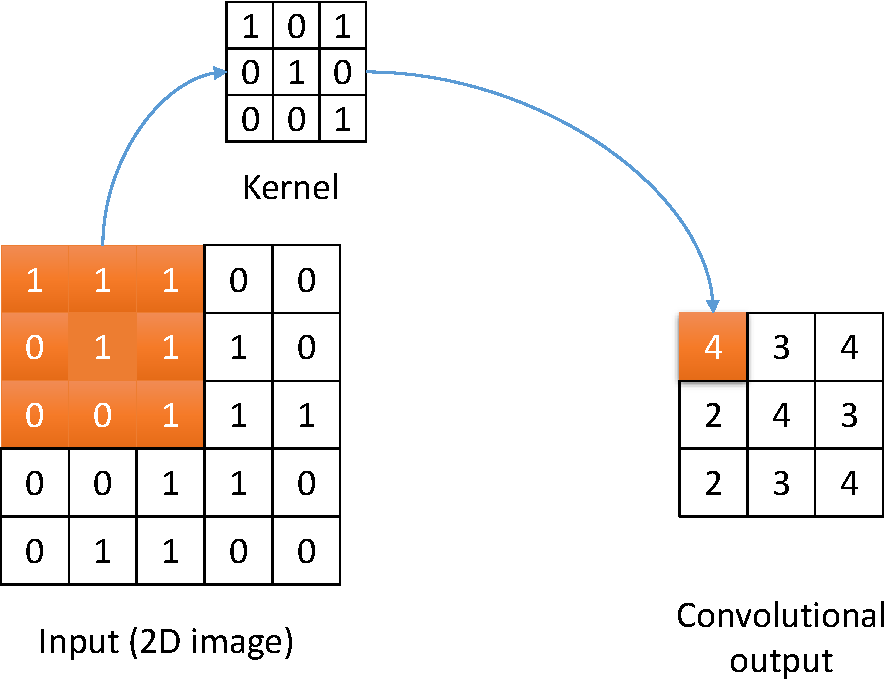
\includegraphics[width=\columnwidth/2]{figures/conv_ops.pdf}
	~ \caption{Simple illustration for convolution. The input is a 2D image, the output is obtained by sliding the kernel through the image.}  
	~ \label{fig:conv_ops}
	~ \end{figure}


\paragraph{Forward propagation} For the purpose of simplicity, in the following operations, we derive the forward and backward formulas for 2D inputs and the delay between convolutional kernels is just one unit. 

In order to mathematically formulate the convolutional layer, let us assume that the input is a $N \times N$ square neuron layer $X$ which is followed by the convolutional layer. Let the filter ($K$) size be $m x m$, the convolutional output $Y$ will be of size $(N - m + 1) \times (N - m + 1)$. Each unit $Y_{ij}$ in the output layer is computed by summing up the contributions from the input layer which are weighted by the kernel:

\begin{equation}
Y_{ij} = \sum_{a=1}^{m} \sum_{b=1}^{m} K_{ab} \cdot X_{(i+a)(j+b)}
\label{eq:convolution}
\end{equation}


The convolutional outputs are usually fed into non-linear functions in a similar manner to the fully-connected layers. In the convolutional layer, we specify the kernels as~\textbf{learnable parameters} which are automatically adjusted during training based on the task of the network.  For example, in the image classification tasks, CNNs have been found to be able to extract from low level features such as edges, colors, shapes to higher-level features such as facial shapes~\cite{krizhevsky2012imagenet}. 

\paragraph{Backward propagation} Let us assume that we have the loss function $\mathcal{L}$ and we know the error values at the convolutional output, $dY_{ij}$ (we keep the same notation as previous network types). Based on the output gradients, we want to compute the derivatives of the loss function with respect to the weights $dK_{ij}$ ($i$ and $j$ are arbitrary indices). 

First, using the chain rule, we sum all of the contributions of all expressions in which the variable occurs:

\begin{equation}
dK_{ab} = \sum_{i=1}^{m} \sum_{j=1}^{m} dY_{ij} \cdot  X_{(i+a)(j+b)}
\label{eq:dconv}
\end{equation}

So that we can update the kernel parameters when we receive the back-propagation signal from the convolutional output. Furthermore, we also need to back-propagate the errors back to the convolutional input, in other words computing $dX_{ij}$

\begin{equation}
dX_{ij} = \sum_{a=1}^{m} \sum_{b=1}^{m} K_{ab} \cdot dY_{(i-a+1)(i-b+1)} 
\label{eq:dconv2}
\end{equation}

From Equations~\ref{eq:dconv},\ref{eq:dconv2}, the backward operations can be efficiently implemented as convolutions similar to the forward operations. Also, the formulas also suggest that, we can expand the convolution with~\textbf{padding} the inputs (so that the backward operations make sense for input units which are close to the border) and increasing the~\textbf{stride} of the convolutions. 

\subsection{Hyper parameters for Convolutional Neural Network}

Given the explanation of convolution - which is the connectivity between the neurons in the input layer and output layer, we can decide the number of neurons in the output layer (which has not been explicitly mentioned in the previous sections). The output layer size depends on the following hyper parameters (which are typically tried experimentally, or with a grid-search strategy). 

\begin{itemize}
	\item \textbf{Kernel size} The size of the window that we use to convolves the input. 
	\item \textbf{Convolution depth} it corresponds to the number of kernels (sliding windows that we use to scan the input, each of which learns a different feature of the input. For example, if we use convolutional neural networks to extract features for sentence classification, then multiple kernels can be distributed to learn features related to nouns, verbs or adjectives. 
	\item As mentioned above, we can alter the step which we slide the filter over the input with the parameters~\textbf{stride}. The larger the stride is, the smaller output is produced by convolution.
	\item We can also control the output size by adding zero values to the the borders of the input. For example in Figure~\ref{fig:conv_ops}, the convolution operator was not able to be performed at the index $(1,1)$ unless we pad 2 zero neurons to each dimension (and each side) of the input. In that case, we will obtain an output with the same size as the input.
\end{itemize}

Two hyper-parameters that affect the number of free parameters are kernel size and depth, while the other two control the output size of the layer. 

%\subsection{Convolution neural networks for NLP}





